\documentclass{article}


\usepackage{geometry}
%\geometry{top=1in, bottom=1in, left=1.15in, right=1.15in}
%\geometry{top=1in, bottom=1in, left=1.15in, right=1.15in}
\geometry{top=1in, bottom=1in, left=1.50in, right=1.50in, marginparwidth=18mm, marginparsep=1mm}


\usepackage{graphicx}
\usepackage{fancyhdr}
\usepackage{titlesec}
\usepackage{tocloft}
\usepackage{amsmath}
\usepackage{amssymb}
\usepackage{hyperref}
\usepackage{wrapfig}
\usepackage{lipsum}
\usepackage{marginnote} 

% Fancy headers and footers
\pagestyle{fancy}
\fancyhf{}
\fancyhead[L]{\leftmark}
\fancyhead[R]{\thepage}


\def\RR{ \mathbb{R} }
\def\TT{ \mathcal{T} }


% Chapter and Section Formatting
\titleformat{\chapter}[display]
  {\normalfont\huge\bfseries}{\chaptername\ \thechapter}{20pt}{\Huge}

\titleformat{\section}{\Large\bfseries}{\thesection}{1em}{}
\titleformat{\subsection}{\large\bfseries}{\thesubsection}{1em}{}


% Title page
\title{-
%\ifteacher \\ (Έκδοση για τον δάσκαλο)  \fi 
}
\author{-}
%\date{1 Οκτωβρίου, 2024}
%\author{Γιώργος Σφήκας}
%\title{ΕΙΣΑΓΩΓΗ ΣΤΗ ΦΩΤΟΓΡΑΜΜΕΤΡΙΑ 
%\\ \small Μέρος πρώτο: Μονοεικονική φωτογραμμετρία


% Multilingual and Greek support
\usepackage{polyglossia}
\setdefaultlanguage{greek}
\setotherlanguage{english}
%\newfontfamily\greekfont[Script=Greek]{GFS Artemisia}
%\newfontfamily\greekfont[Script=Greek]{GFS Didot}
%\newfontfamily\greekfont[Script=Greek]{GFS Bodoni}
%\newfontfamily\greekfont[Script=Greek]{GFS Neohellenic}
%\newfontfamily\greekfont[Script=Greek]{GFS Solomos}
%\newfontfamily\greekfont{DejaVu Serif}
%\newfontfamily\greekfont{DejaVu Sans}
%\newfontfamily\greekfont{Times New Roman}
%\newfontfamily\greekfont{FreeSerif}
\newfontfamily\greekfont{FreeSans}
%\newfontfamily\greekfont{Fira Sans}

%\newfontfamily\greekfont{Libertinus Serif}
%\newfontfamily\greekfont{EB Garamond}


\begin{document}
% \author{Ακαδημαϊκό έτος: 2025-2026\\
% Τμήμα Μηχανικών Τοπογραφίας και Γεωπληροφορικής\\
% Διδάσκων: Γιώργος Σφήκας\\
% \\
% Ημερομηνία παράδοσης: Παρασκευή 14 Νοεμβρίου}
% \title{Γραφικά Υπολογιστών ($GEO820$)\\
% 1η σειρά ασκήσεων\\}

% \date{}
%\maketitle

\section*{Σύντομη περιγραφή κώδικα για μη καταστροφική σήμανση}

\begin{figure}[ht]
    \centering
    \begin{tabular}{cc}
        
\includegraphics[width=0.45\textwidth]{../fixtures/IMG_7327.JPG} &
        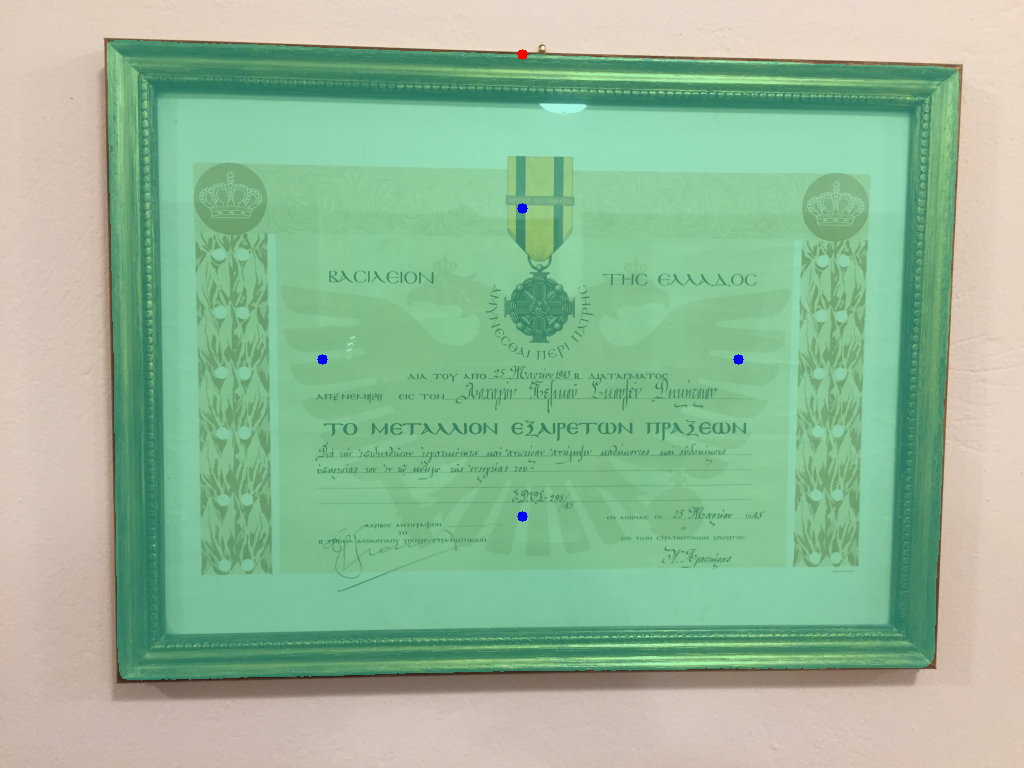
\includegraphics[width=0.45\textwidth]{overlays/IMG_7327_overlay.png} \\

        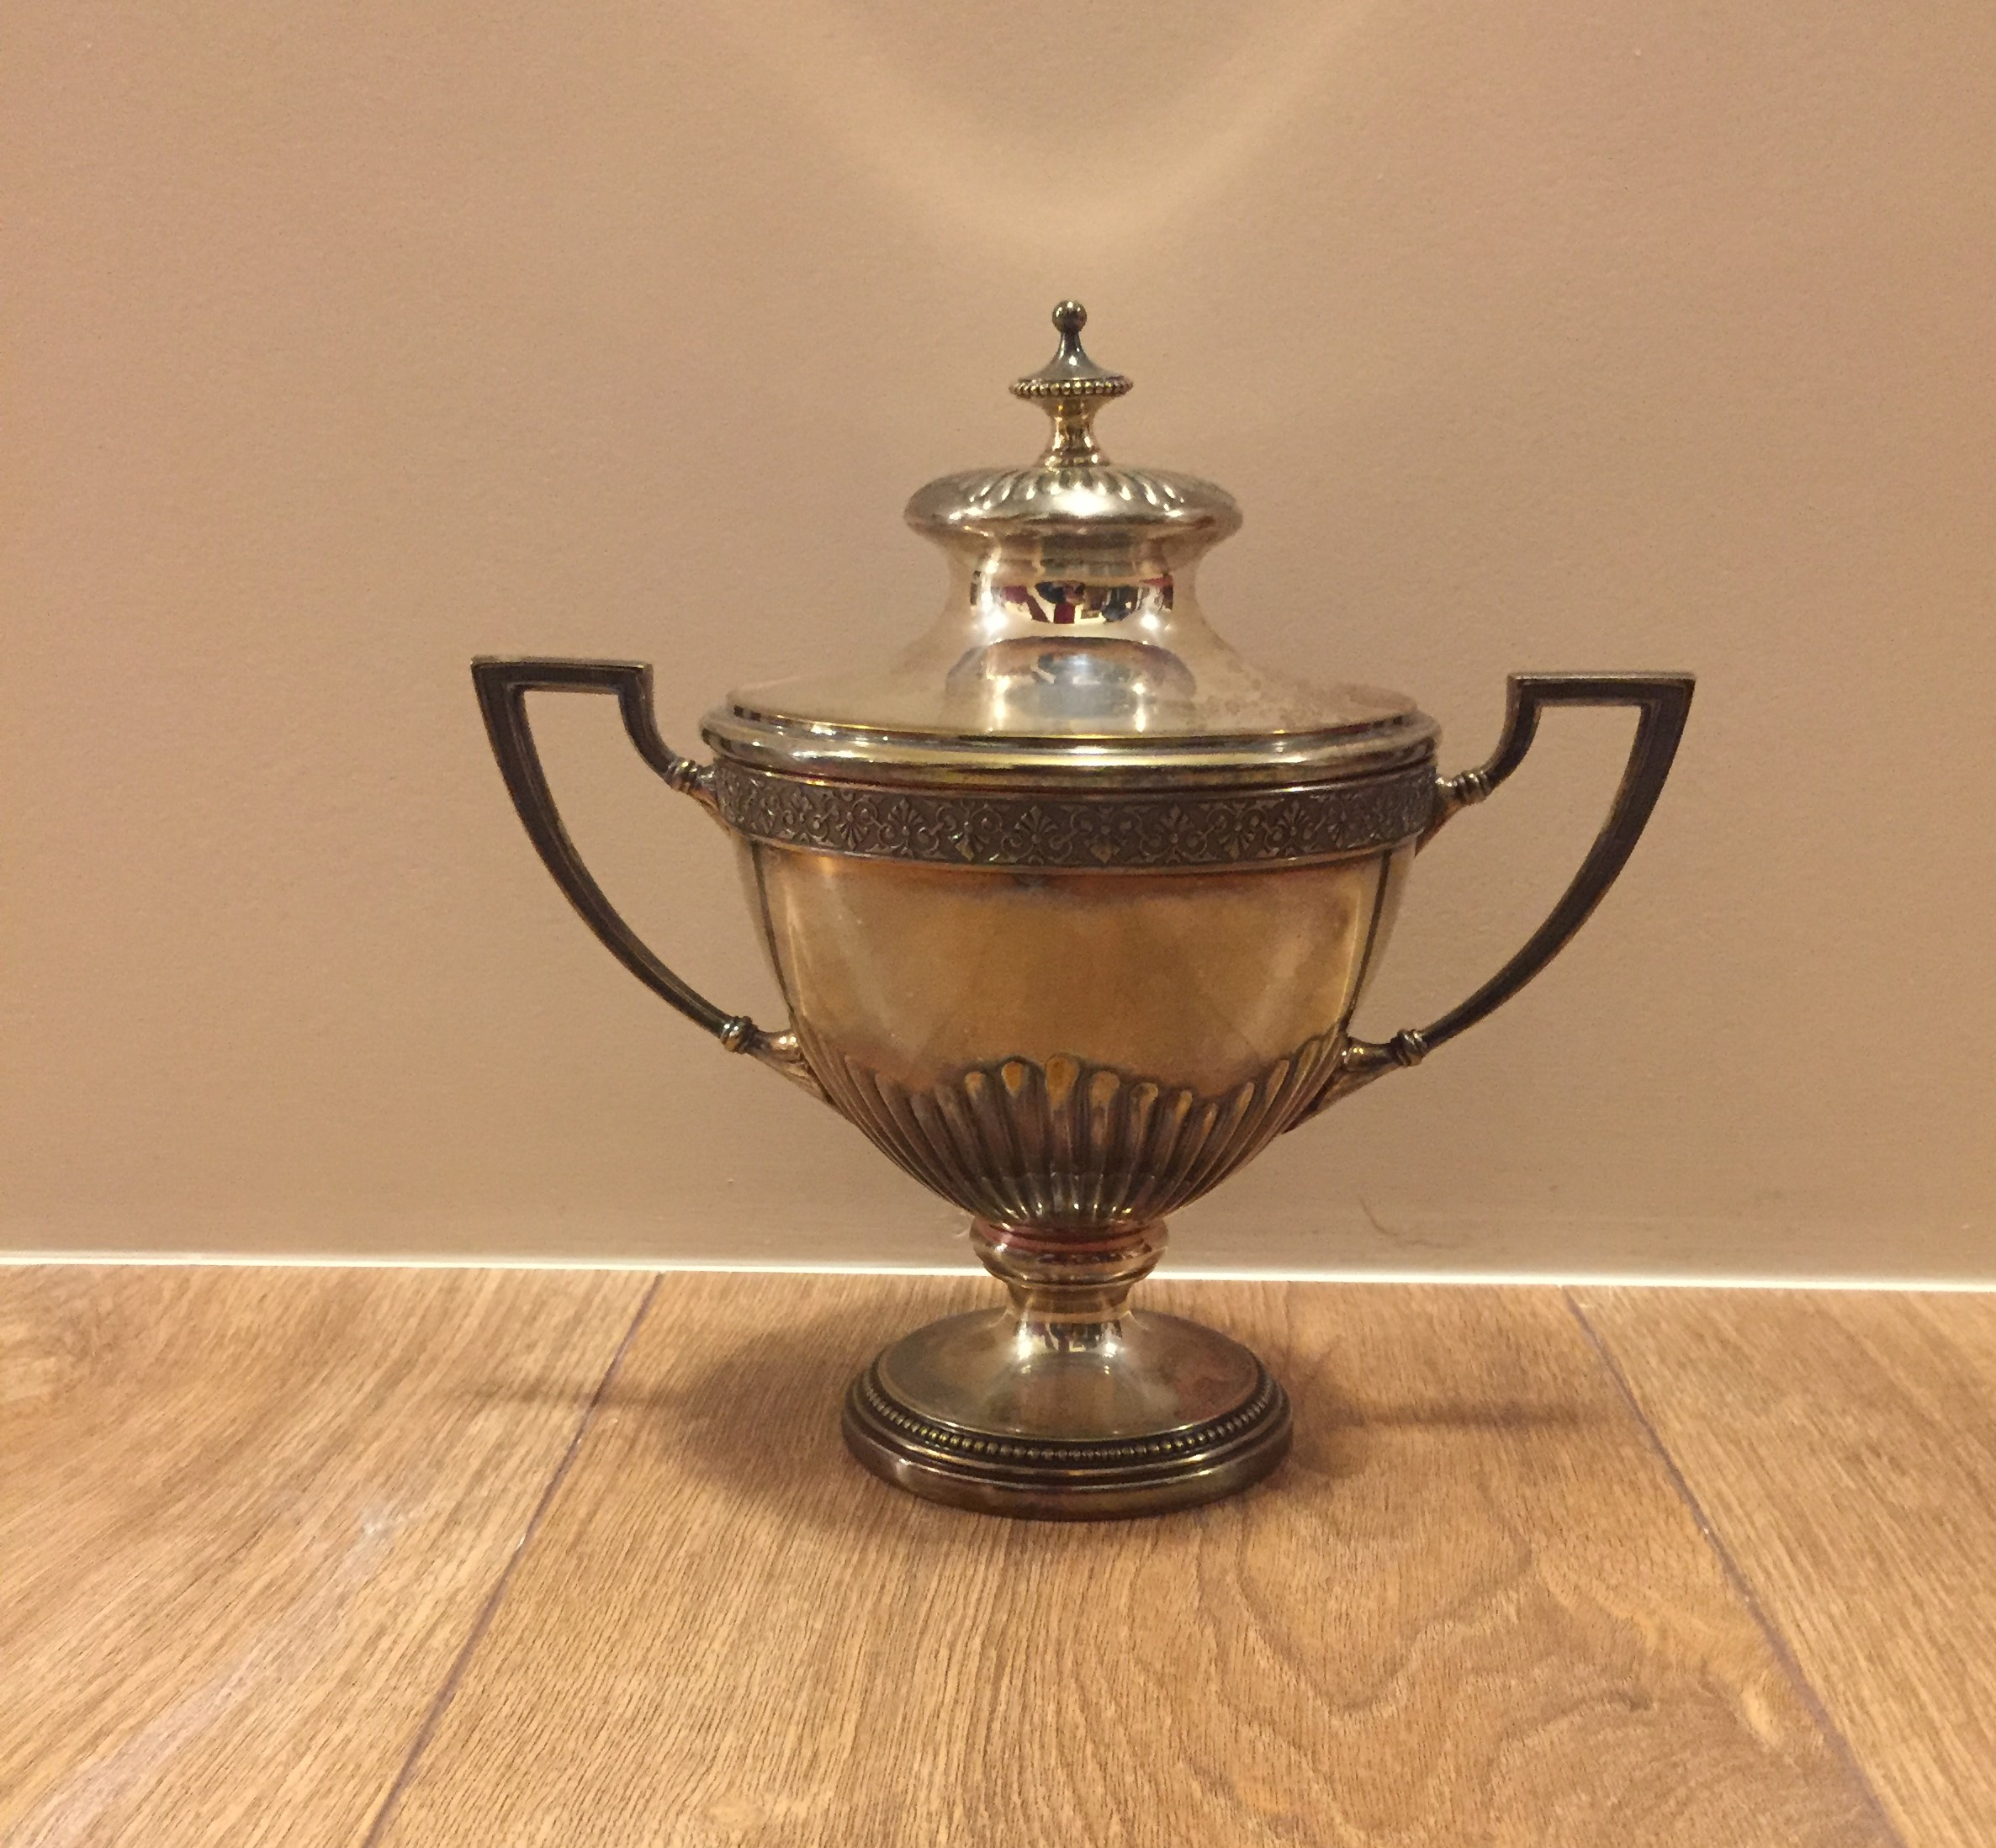
\includegraphics[width=0.45\textwidth]{../fixtures/IMG_7343.JPG} &
        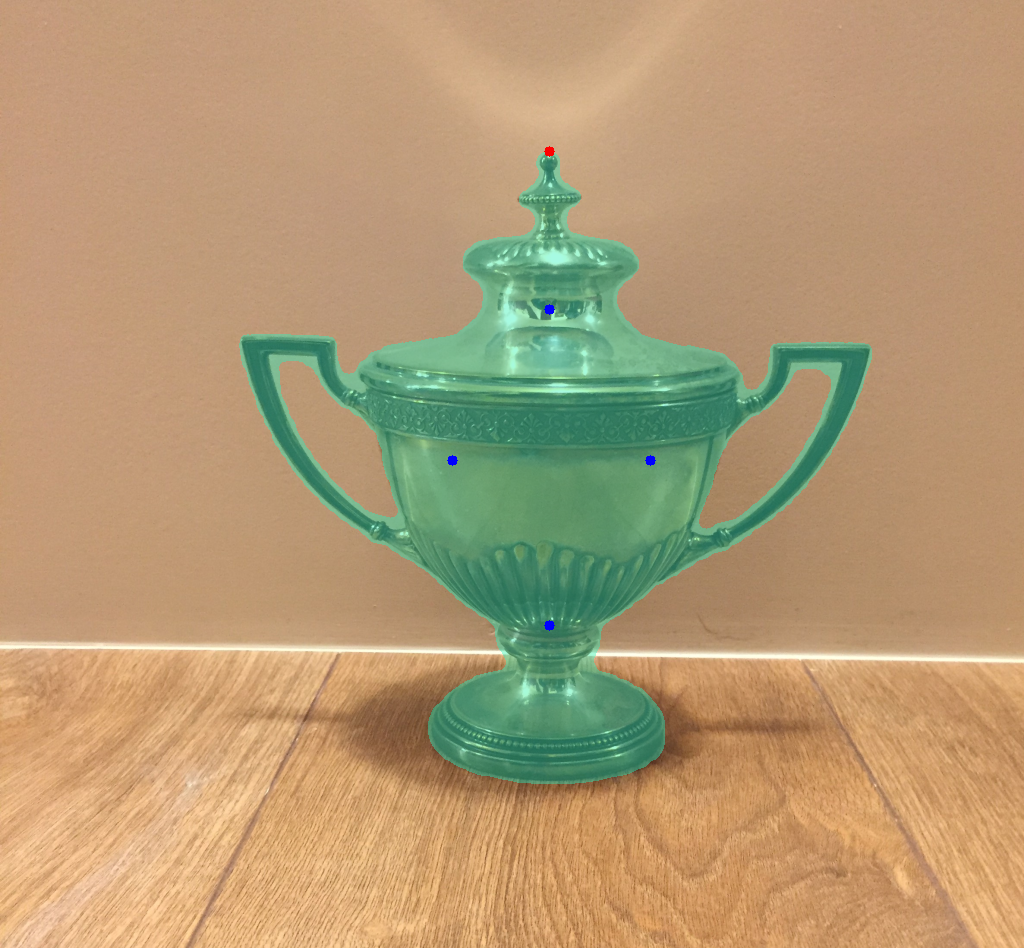
\includegraphics[width=0.45\textwidth]{overlays/IMG_7343_overlay.png} \\

        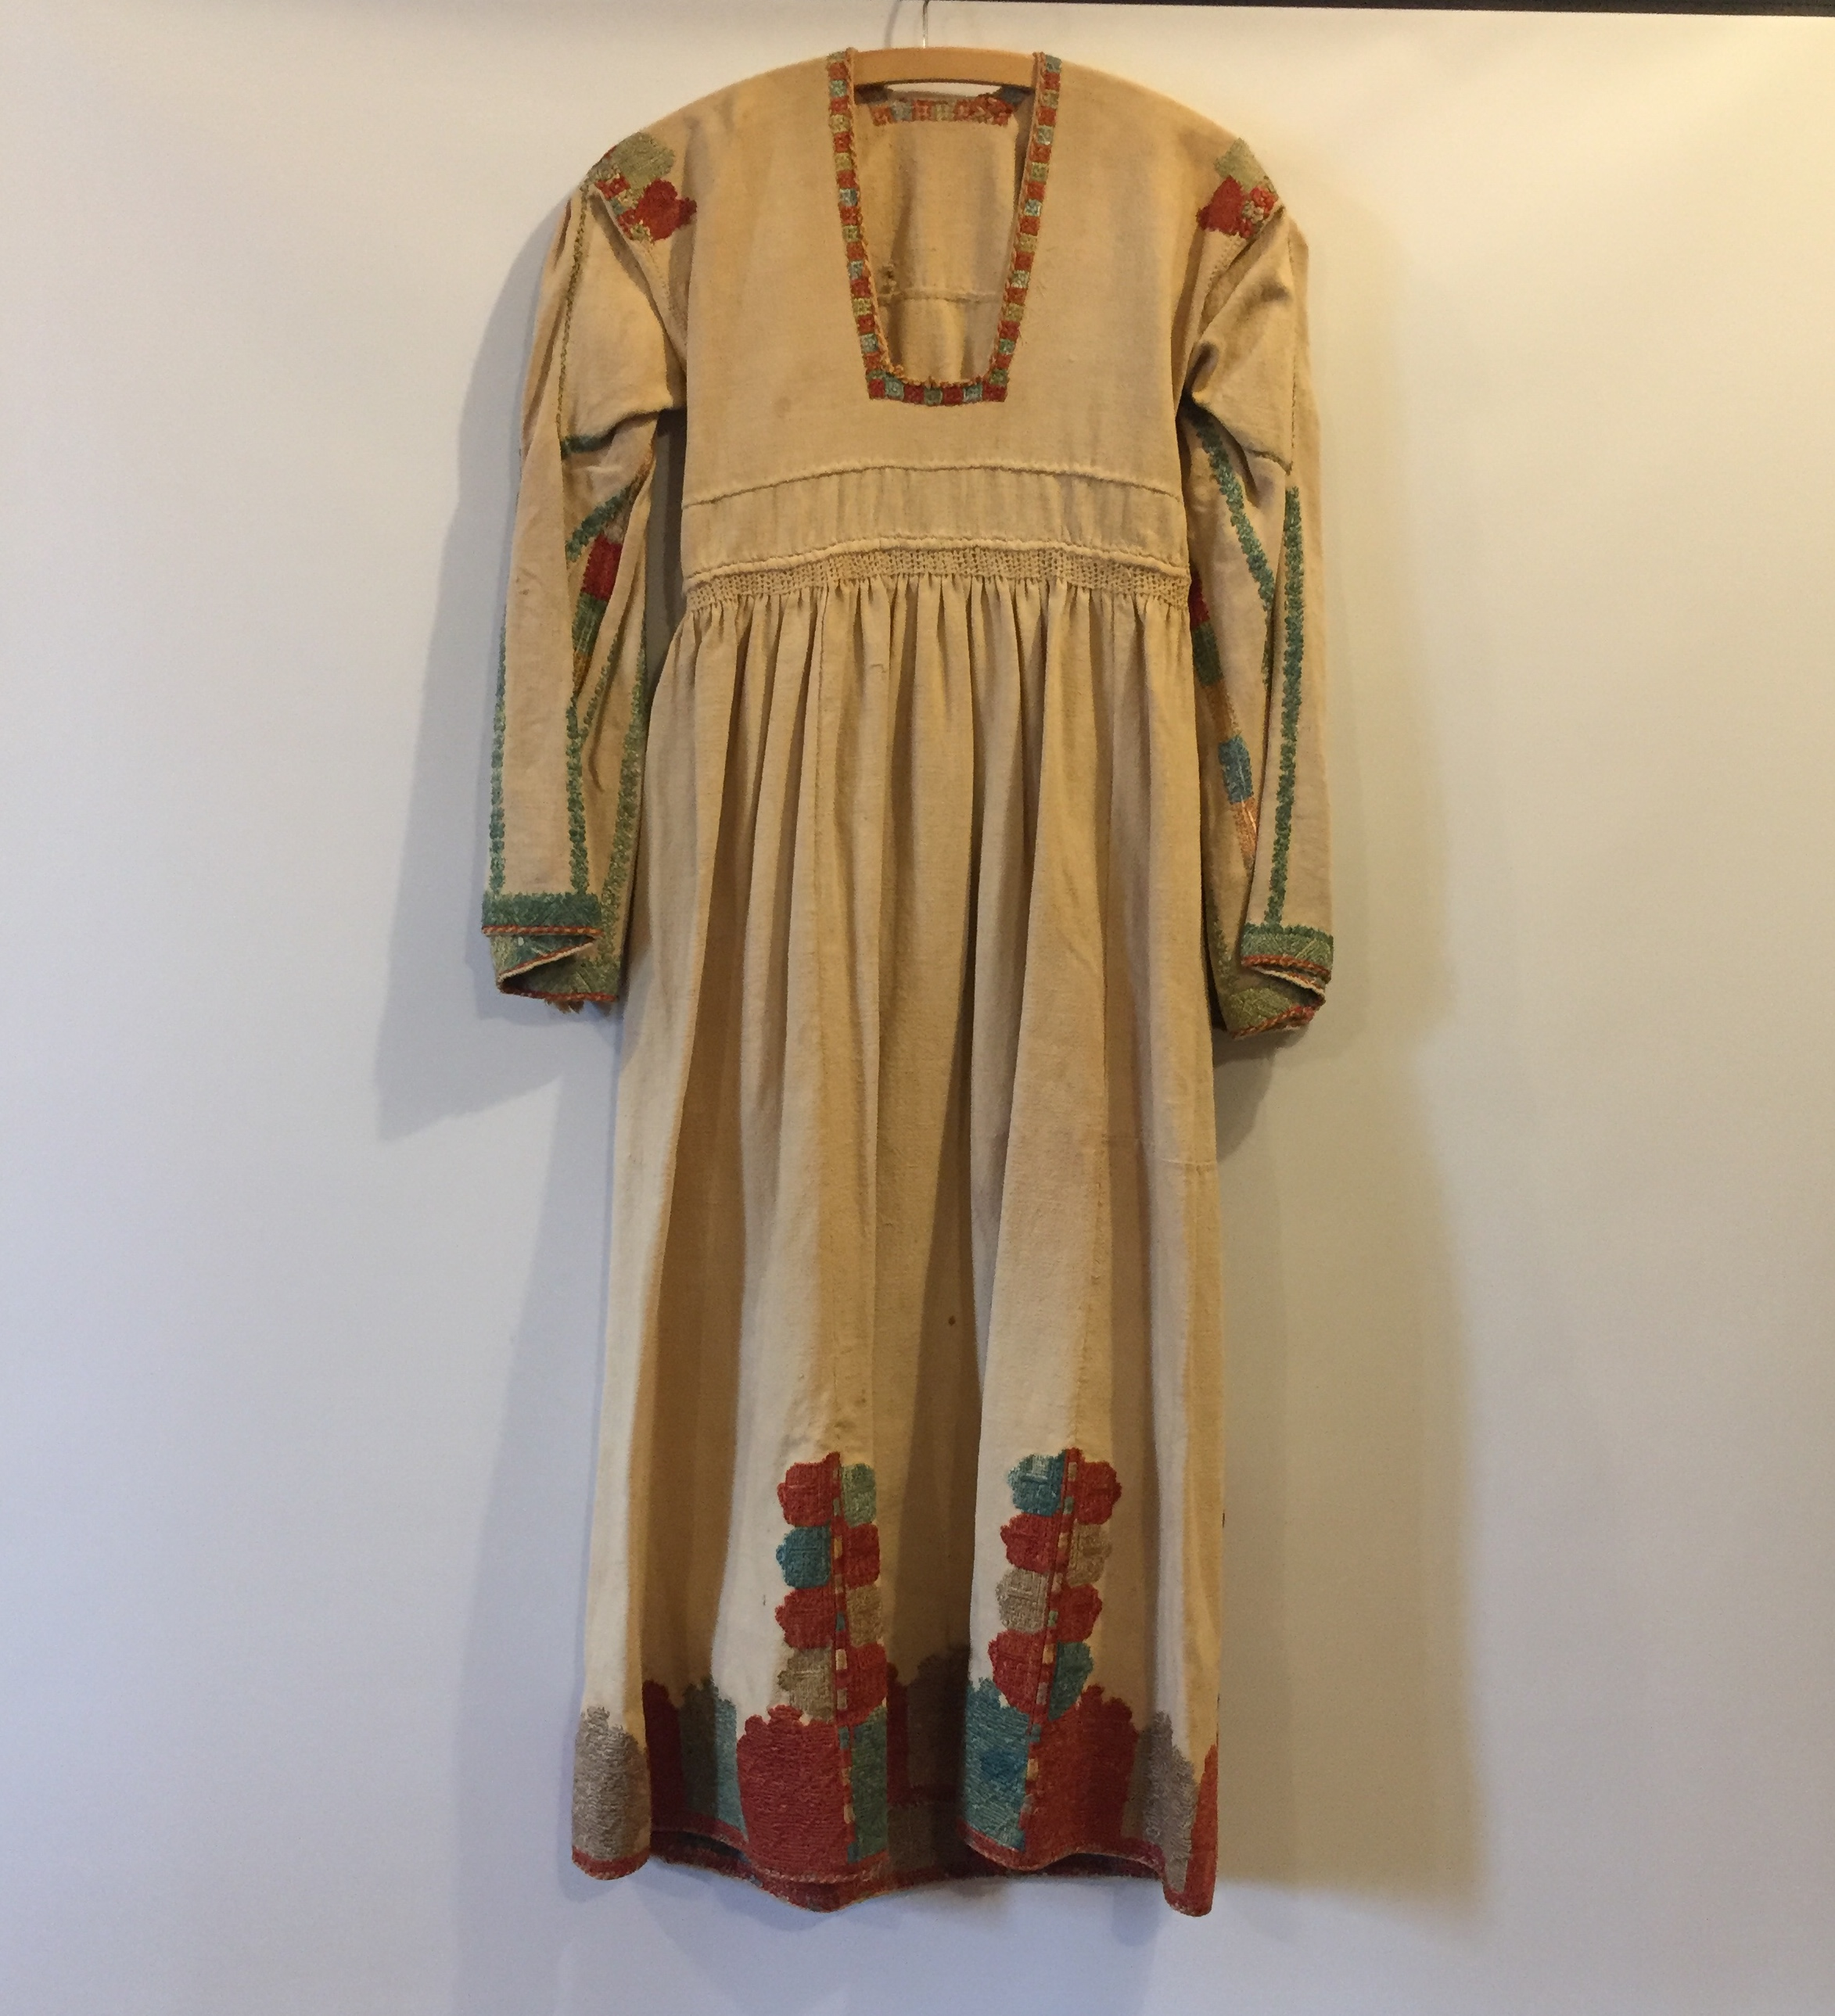
\includegraphics[width=0.45\textwidth]{../fixtures/IMG_7553.jpg} &
        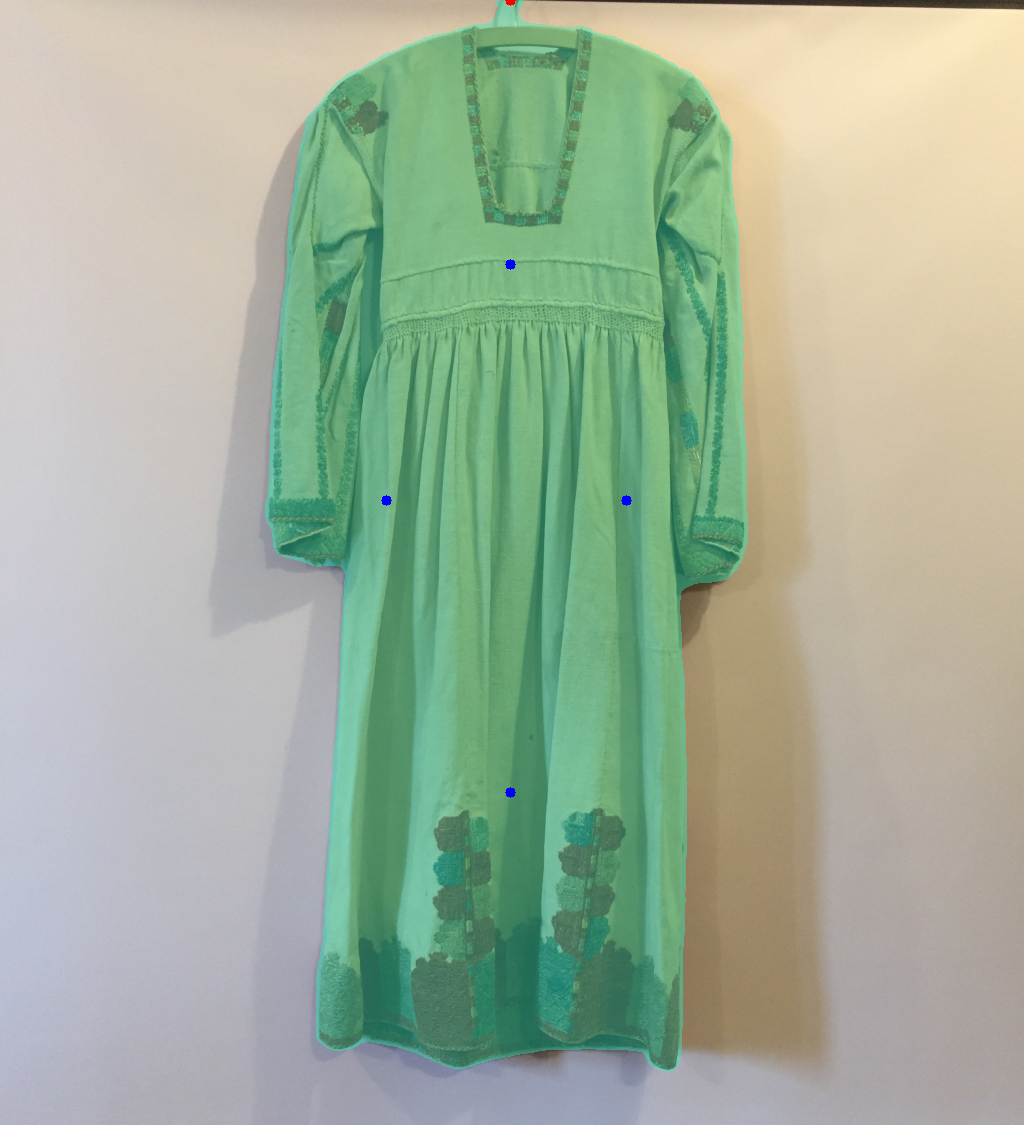
\includegraphics[width=0.45\textwidth]{overlays/IMG_7553_overlay.png} \\

        \includegraphics[width=0.45\textwidth]{../fixtures/IMG_20221129_145349.jpg} &
        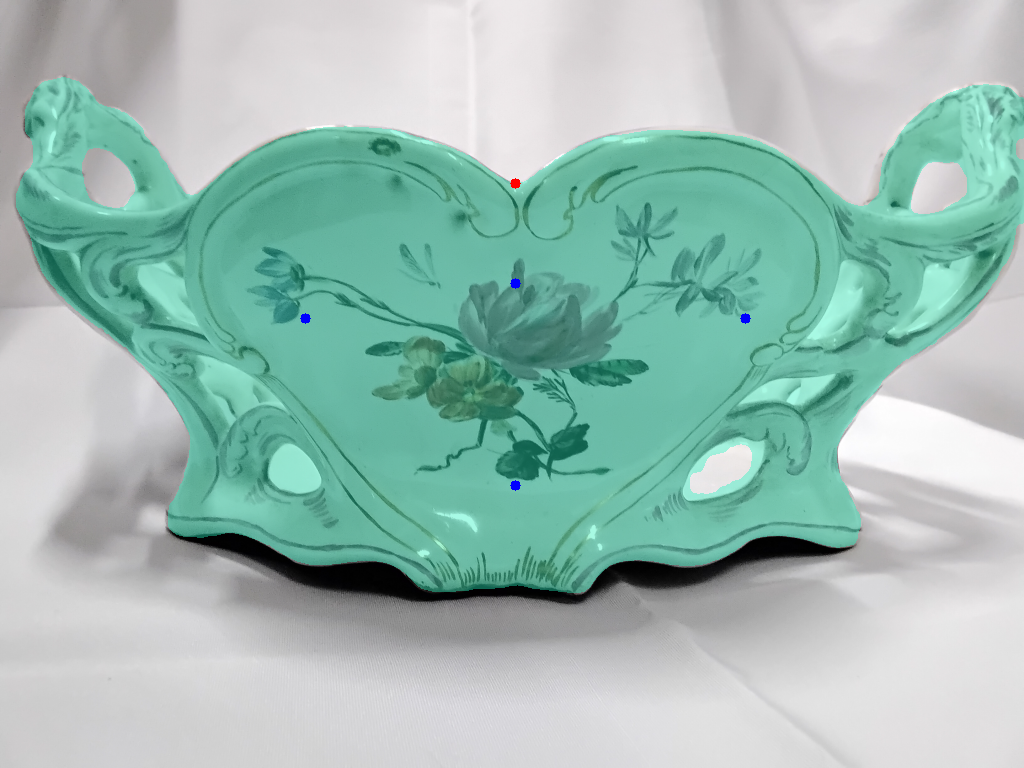
\includegraphics[width=0.45\textwidth]{overlays/IMG_20221129_145349_overlay.png} \\
    \end{tabular}
    \caption{ 
    \label{table:qualitative1}
    Δείγμα αποτελέσματος εκτέλεσης (μέρος 1ο). Στην αριστερή εικόνα έχουμε τις πρωτότυπες εικόνες,
    ενώ στην δεξιά φαίνονται οι ίδιες εικόνες με την αυτόματη επισημείωση που παρήγαγε ο κώδικας μας.
    }
\end{figure}

\begin{figure}[ht]
    \centering
    \begin{tabular}{cc}
        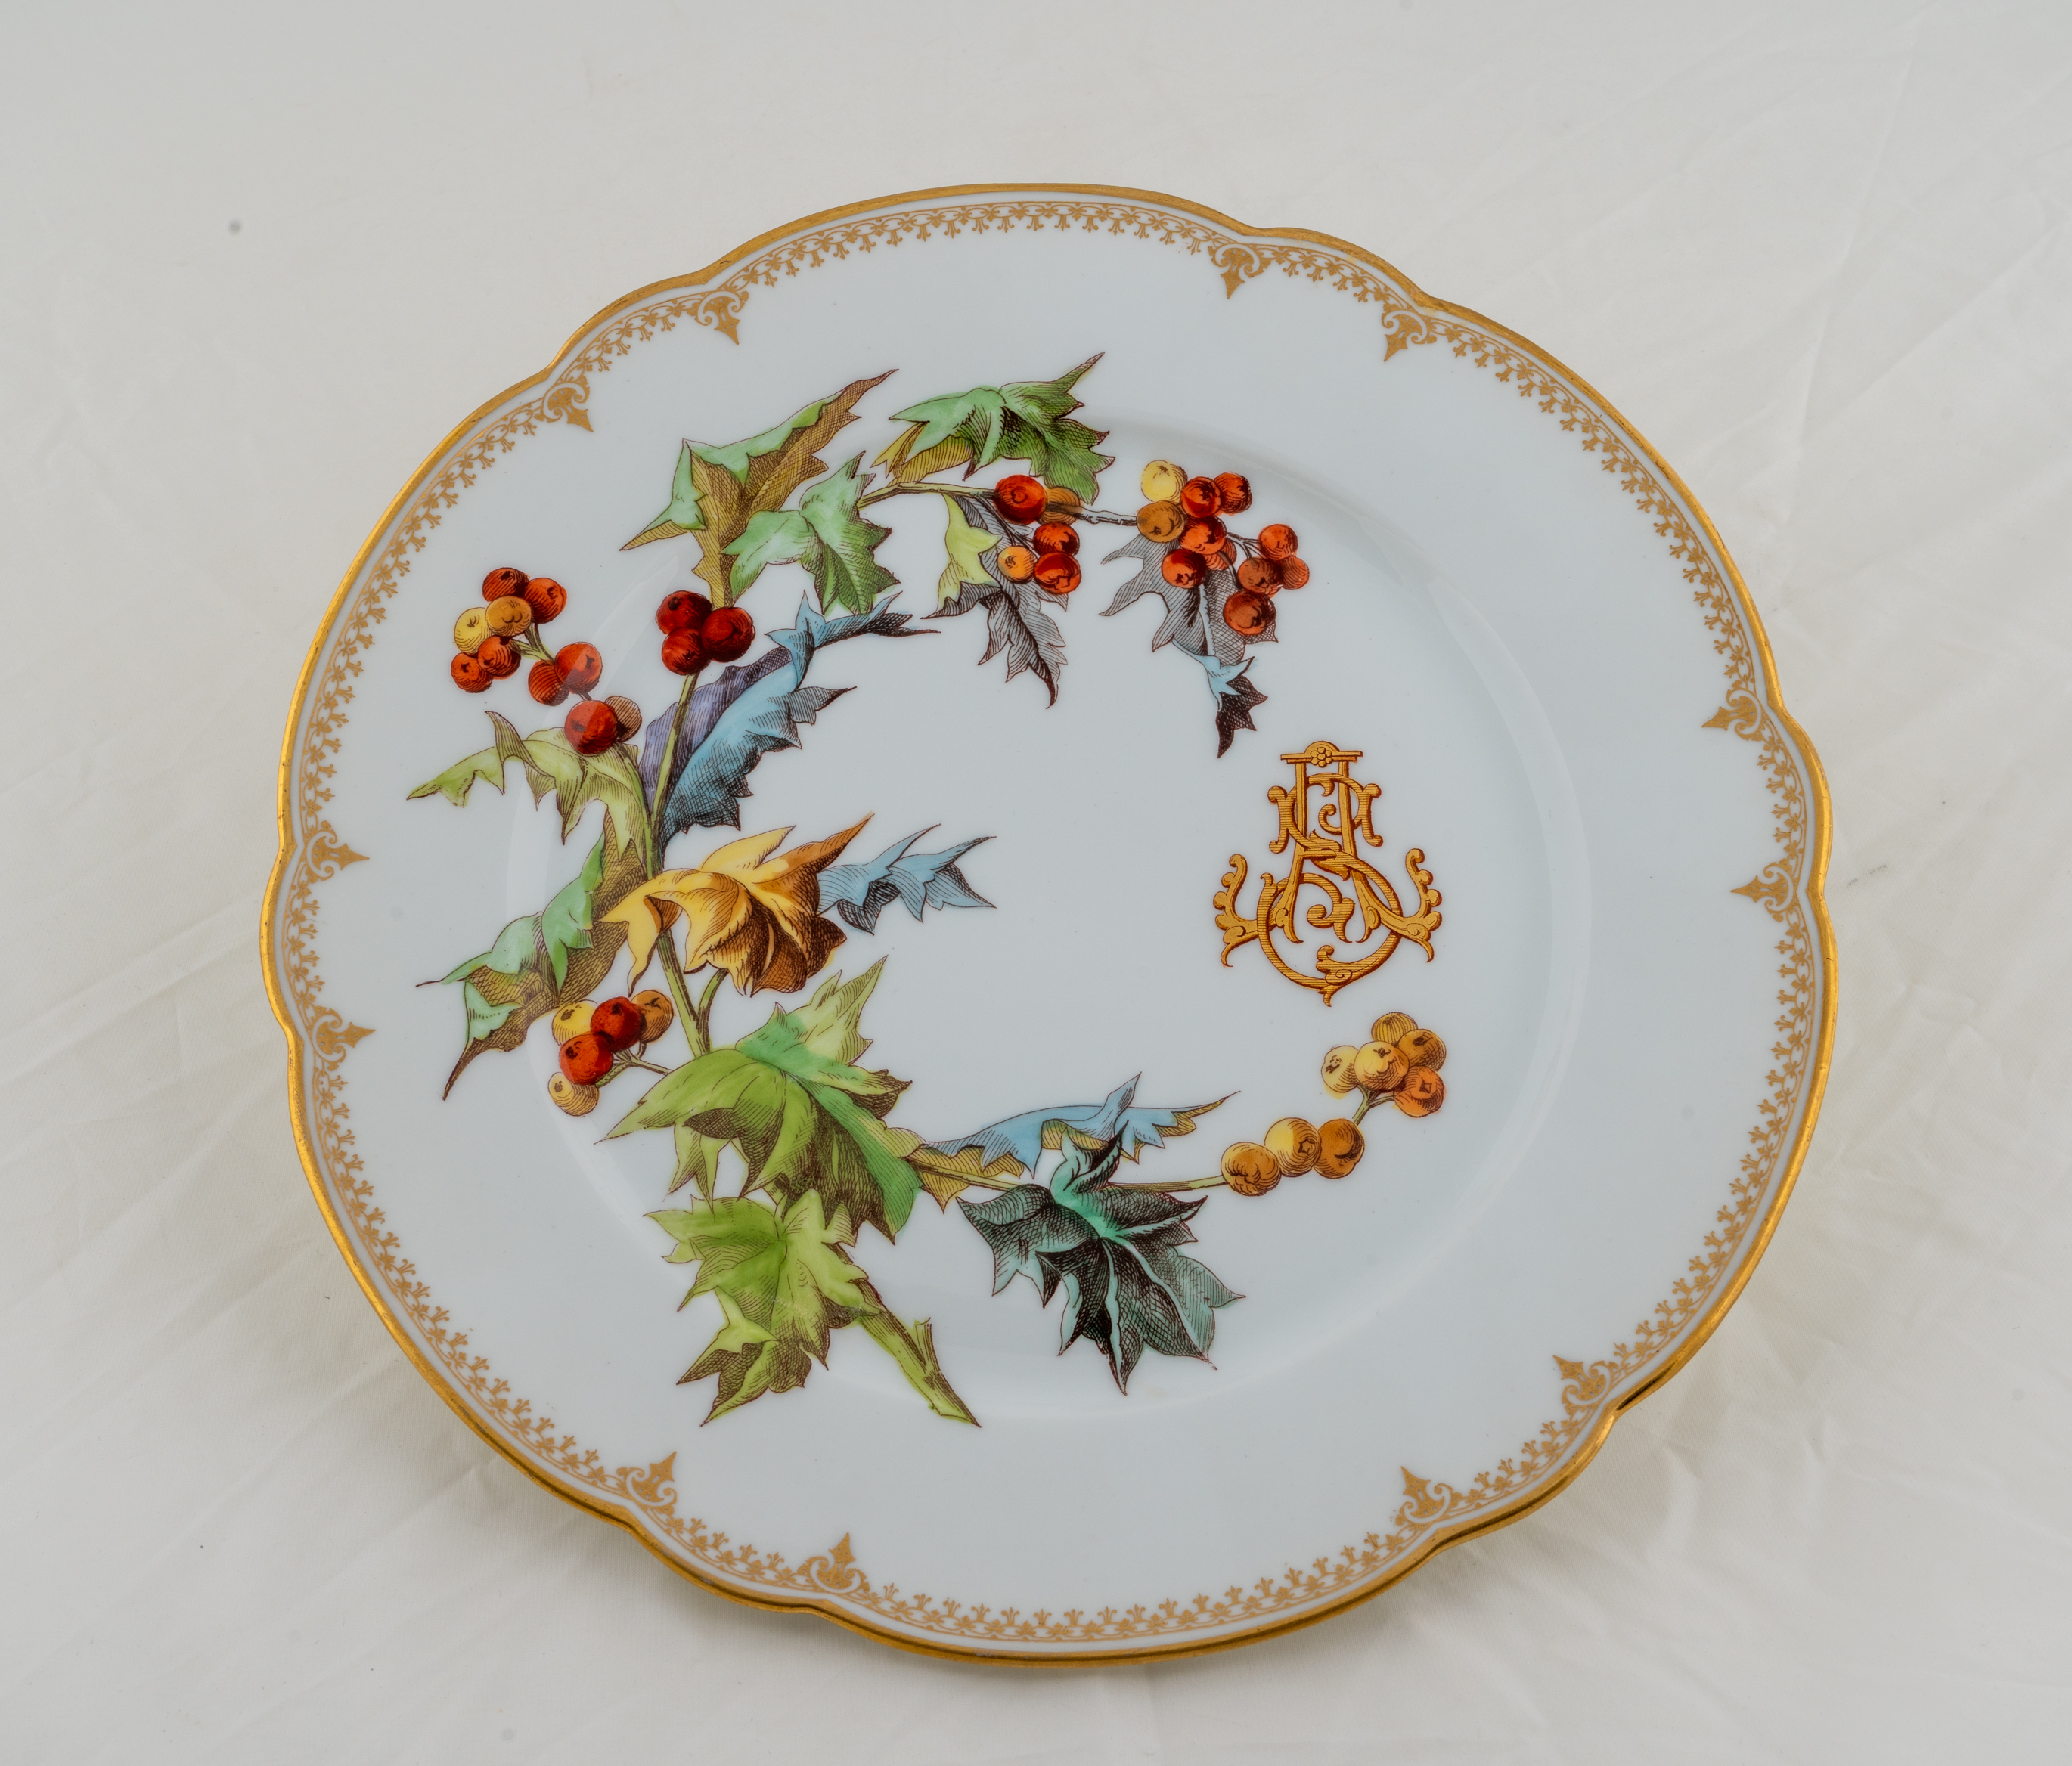
\includegraphics[width=0.45\textwidth]{../fixtures/sa-low-052.jpg} &
        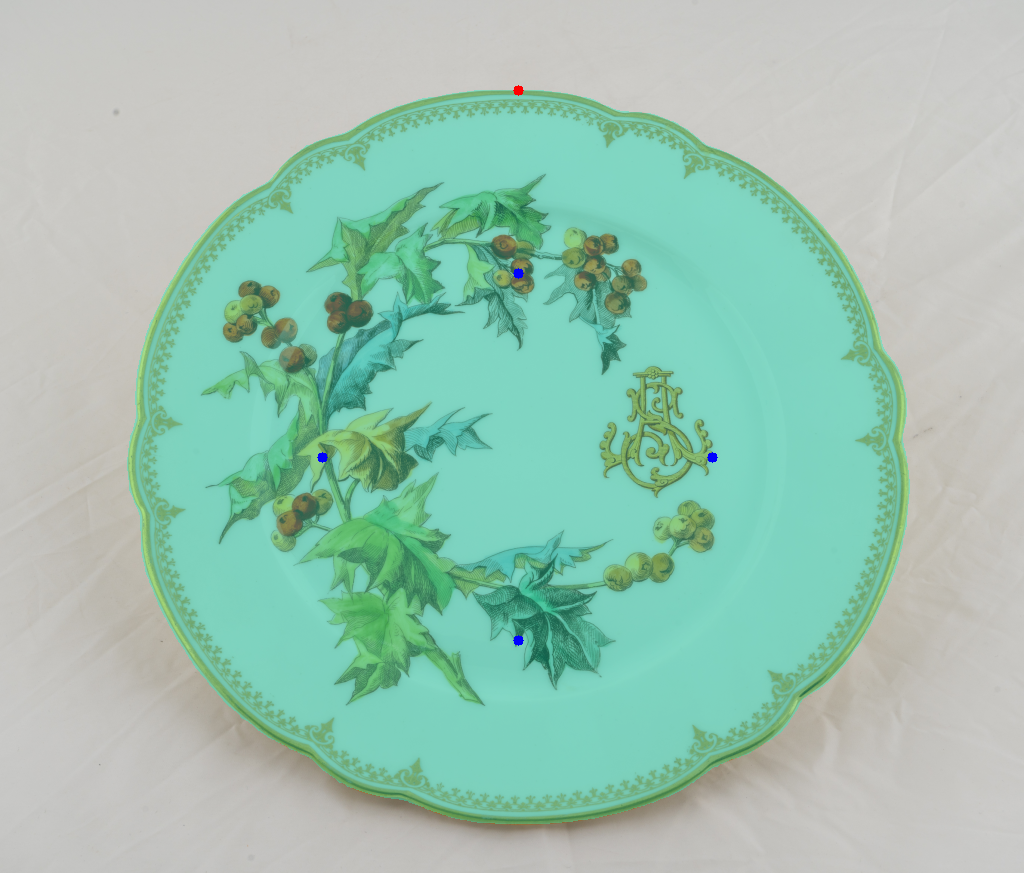
\includegraphics[width=0.45\textwidth]{overlays/sa-low-052_overlay.png} \\

        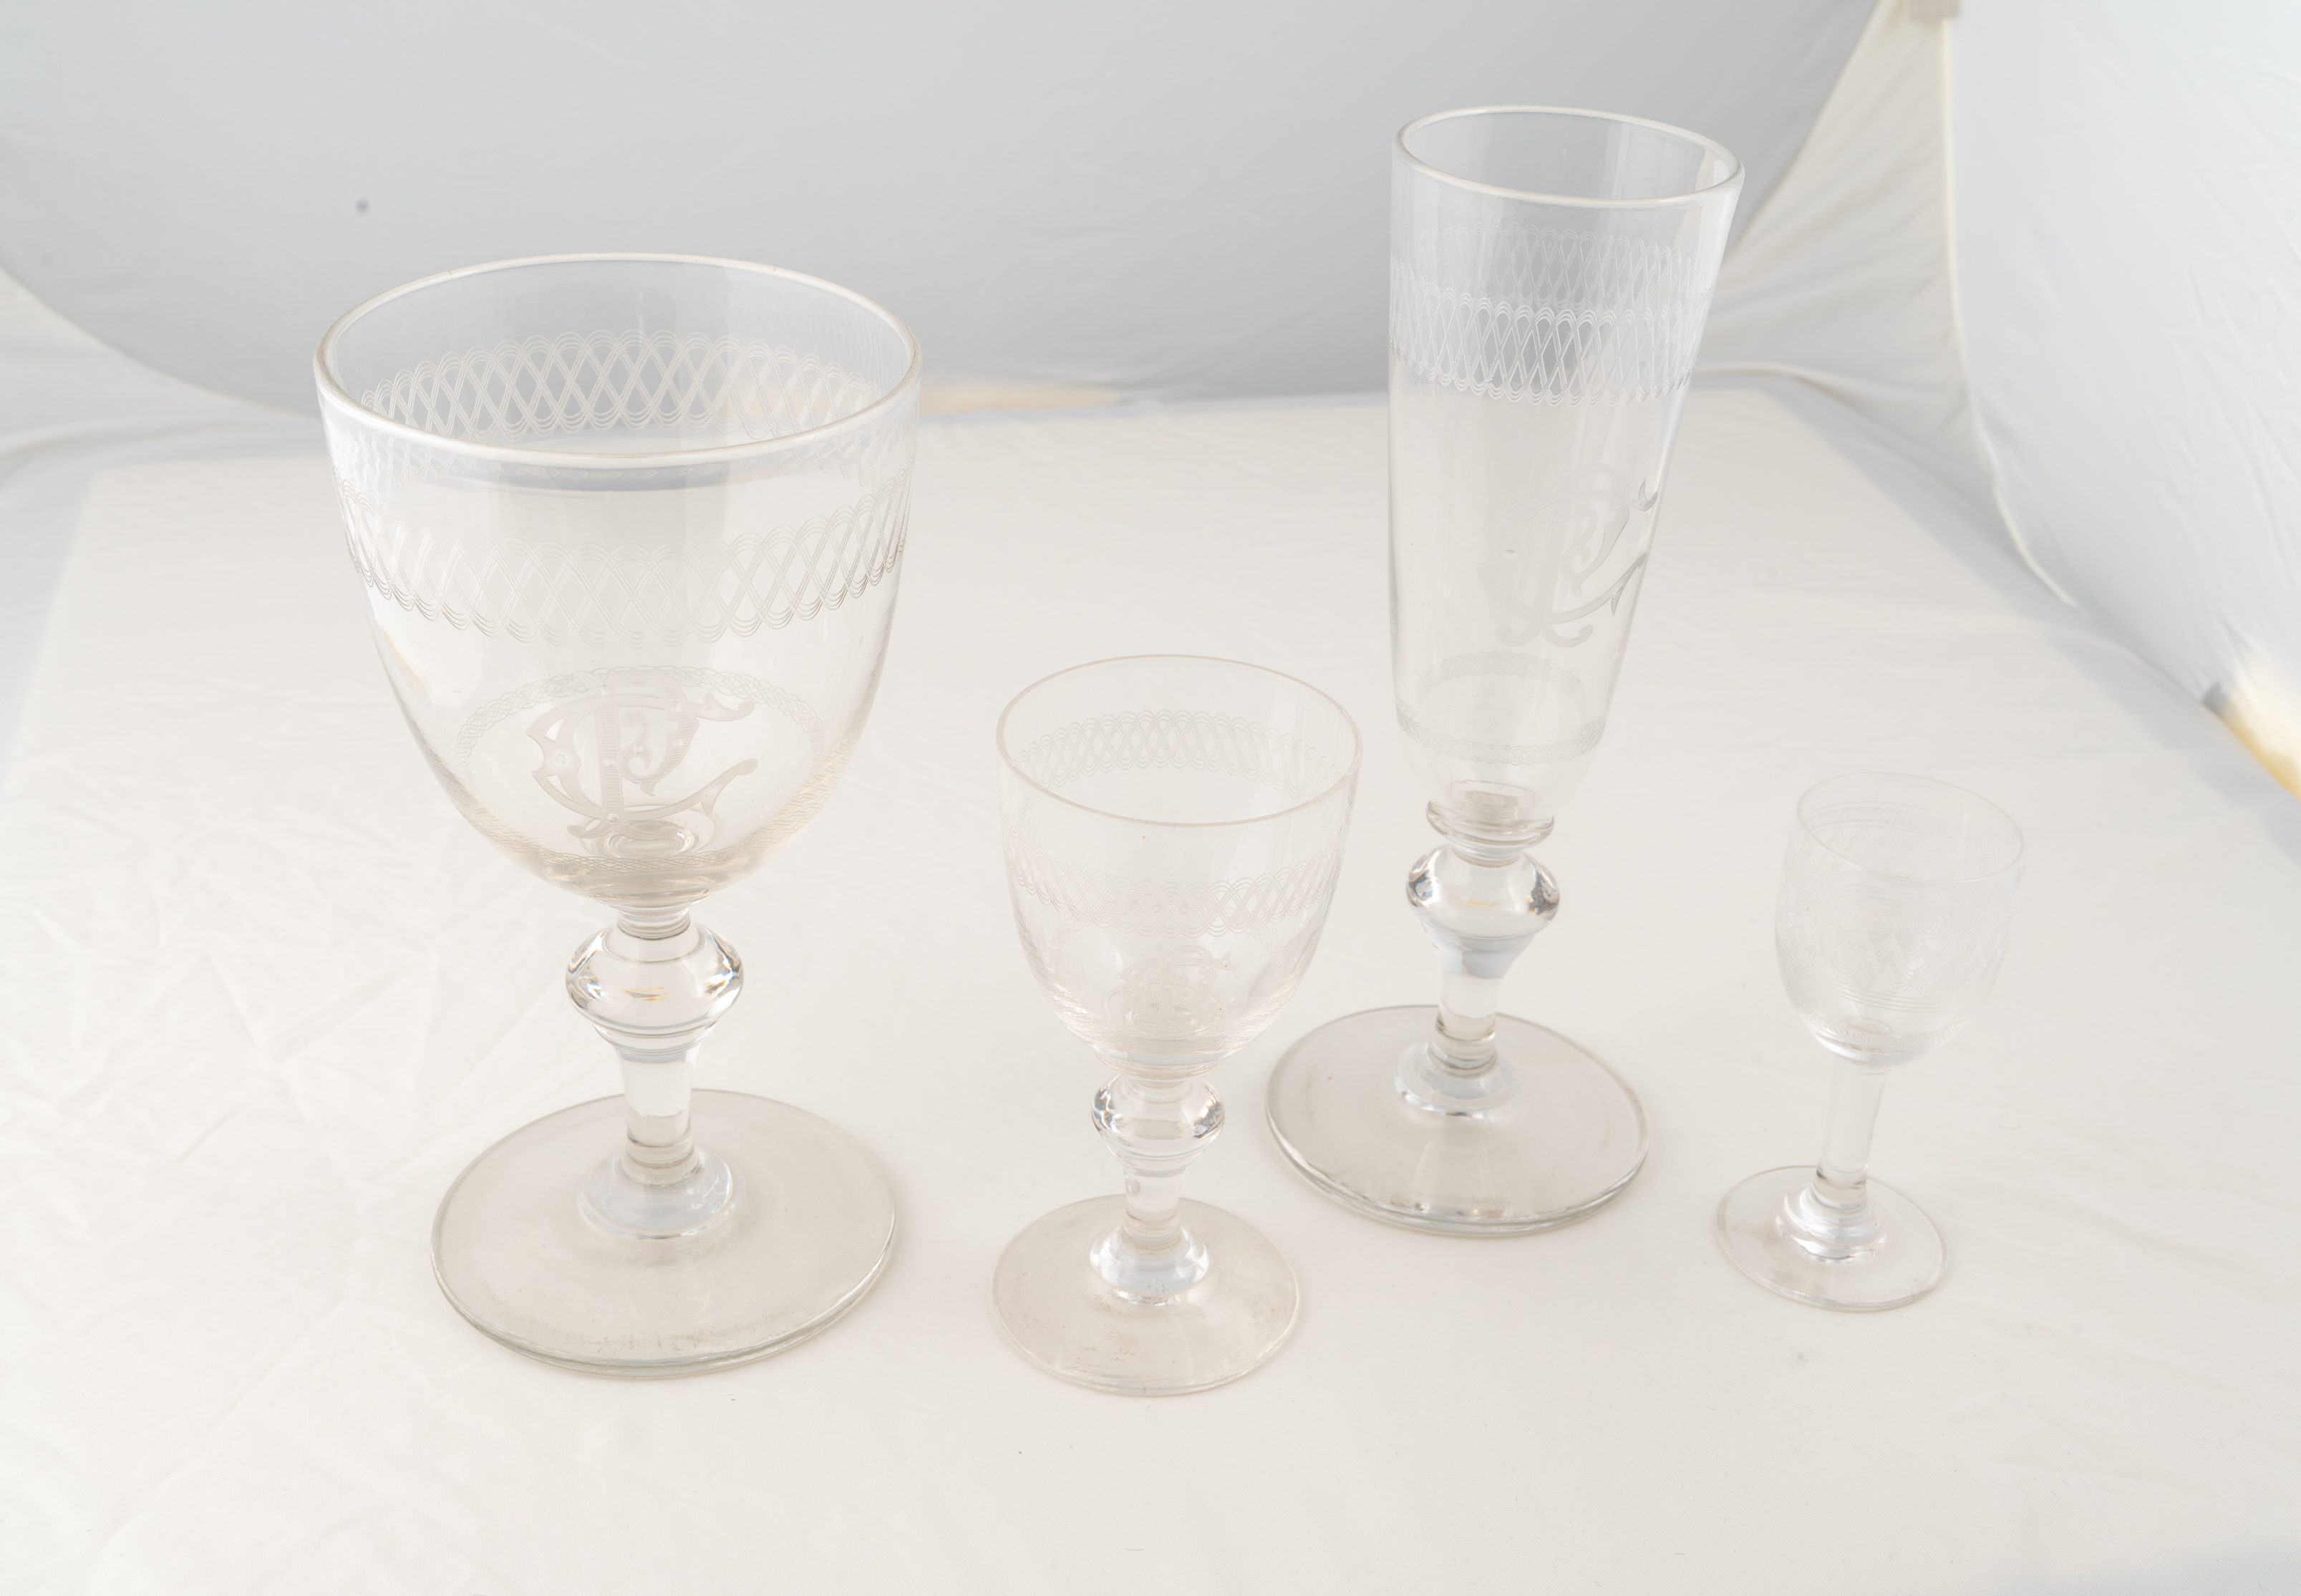
\includegraphics[width=0.45\textwidth]{../fixtures/sa-low-123.jpg} &
        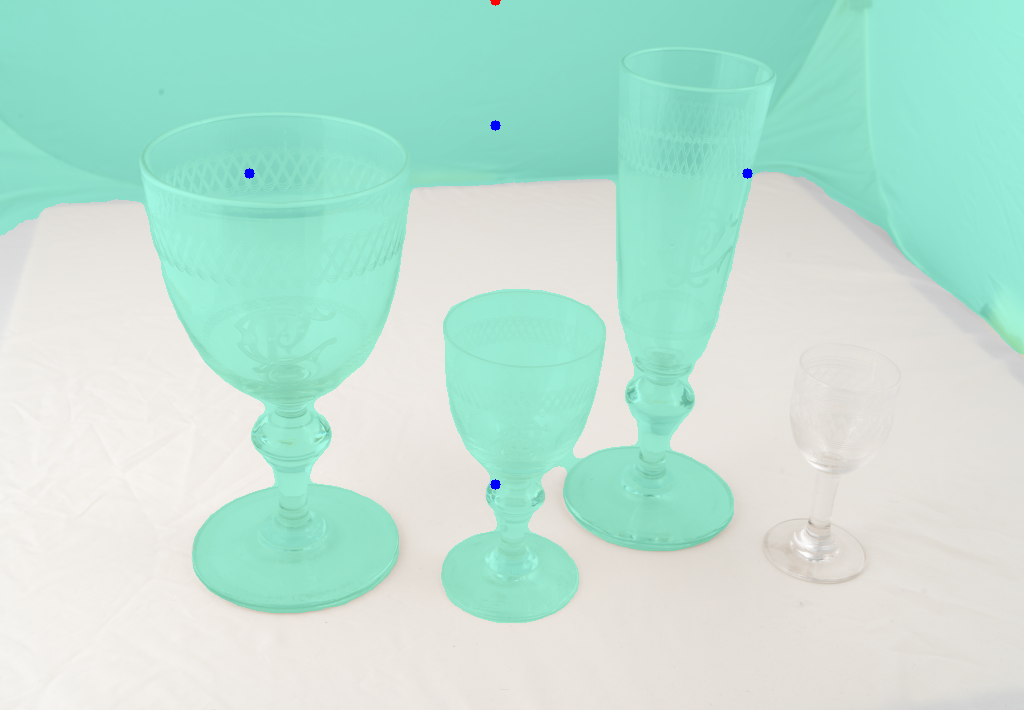
\includegraphics[width=0.45\textwidth]{overlays/sa-low-123_overlay.png} \\

        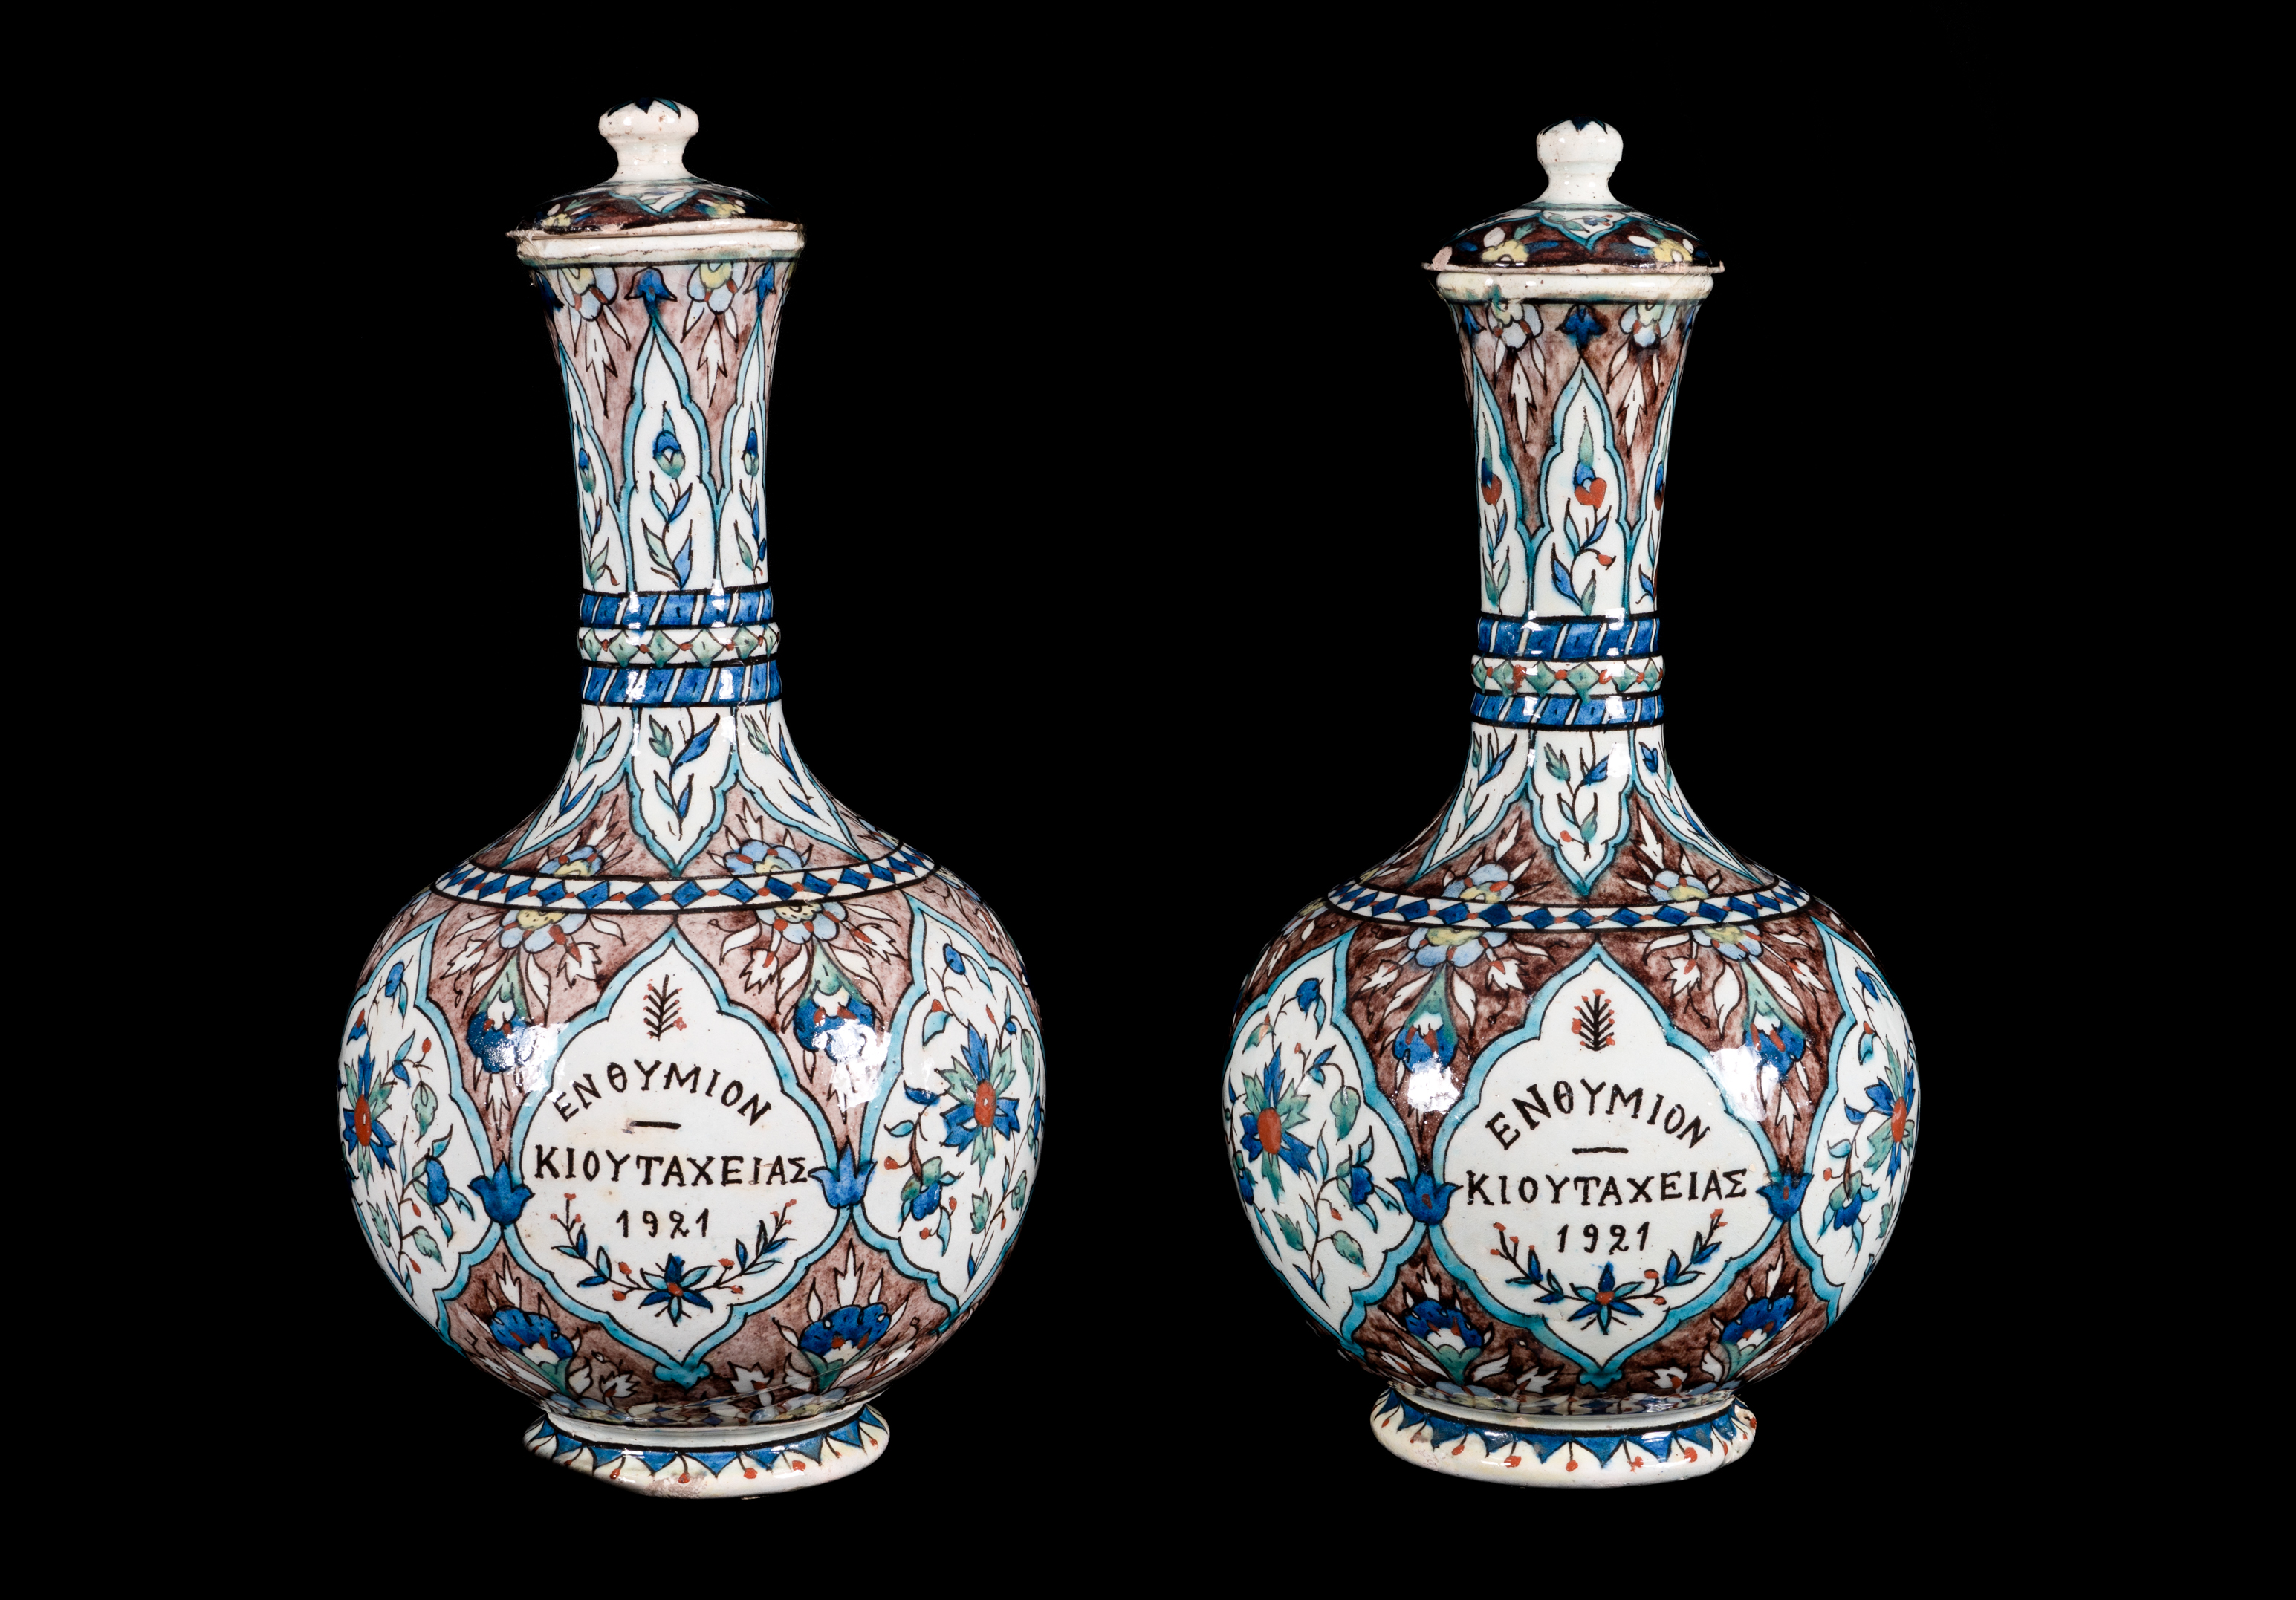
\includegraphics[width=0.45\textwidth]{../fixtures/sa-low-160.jpg} &
        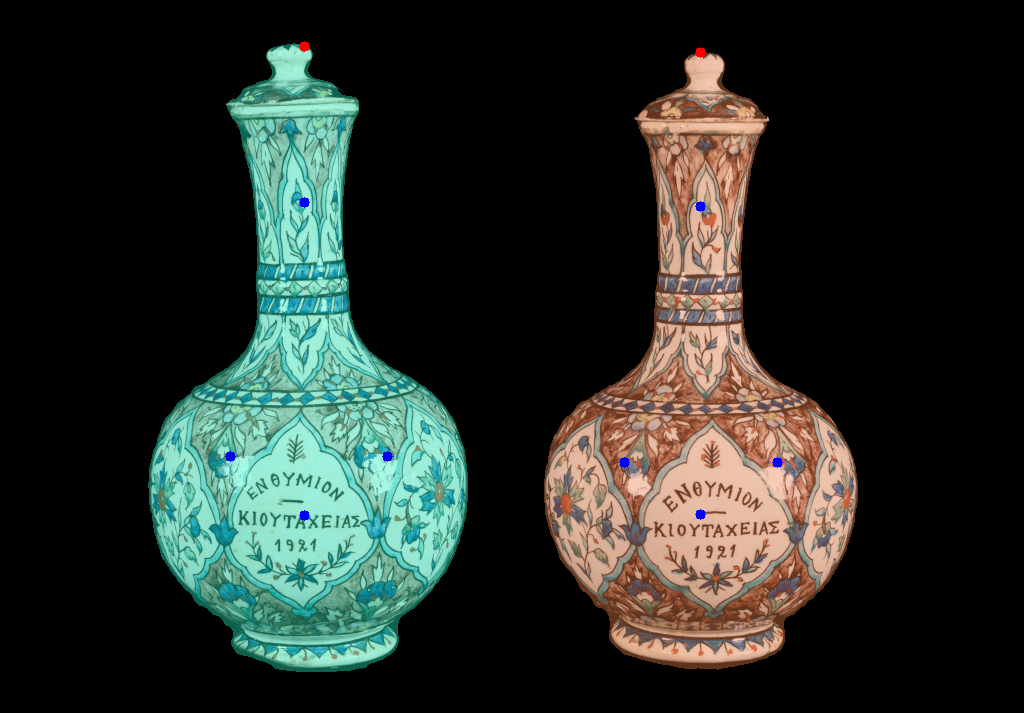
\includegraphics[width=0.45\textwidth]{overlays/sa-low-160_overlay.png} \\
    \end{tabular}
    \caption{ 
    \label{table:qualitative2}
    Δείγμα αποτελέσματος εκτέλεσης (μέρος 2ο). Στην αριστερή εικόνα έχουμε τις πρωτότυπες εικόνες,
    ενώ στην δεξιά φαίνονται οι ίδιες εικόνες με την αυτόματη επισημείωση που παρήγαγε ο κώδικας μας.
    Στην δεύτερη γραμμή φαίνεται μια περίπτωση όπου μπορεί να υπάρξει σφάλμα -- τα αντικείμενα πρέπει να τοποθετούνται σε σχέση
    με μη ομοιόμορφο φόντο, και ο αριθμός τους να είναι όσο το δυνατόν μικρότερος ανά λήψη.
    }
\end{figure}

Ο τρόπος εκτέλεσης του κώδικα έχει ως εξής. Αφού ολοκληρωθεί η εγκατάσταση των απαραίτητων πακέτων Python,
τρέχουμε το εκτελέσιμο εισάγοντας τις παρακάτω παραμέτρους:
\begin{itemize}
    \item $-i$: Δίνουμε το όνομα αρχείου της εικόνας που θέλουμε να επεξεργαστούμε.
    \item $--numVerticalPoints$: Αριθμός σημείων επί της "μεσοκαθέτου". Μπορούν να είναι το πολύ 2. (Προαιρετική παράμετρος, default value = 1)
    \item $--numGeneralPoints$: Αριθμός σημείων εκτός "μεσοκαθέτου". Μπορούν να είναι το πολύ 4. (Προαιρετική παράμετρος, default value = 4)
    \item $--debug$: Αν ενεργοποιηθεί, θα αποθηκευτεί το αποτελέσματα ως επισημείωση σε αντίγραφο της πρωτότυπης εικόνας.
\end{itemize}

Το αποτέλεσμα θα τυπωθεί στο τερματικό. Εάν έχει ενεργοποιηθεί η επιλογή "debug", τότε θα αποθηκευτεί επίσης νέα εικόνα όπου θα φαίνεται η παραχθείσα επισημείωση.

Επίσης, μπορεί να χρησιμοποιηθεί η συνάρτηση "pointDetector" ως τμήμα άλλου κώδικα. Η τιμή επιστροφής της είναι οι συντεταγμένες των προτεινόμενων σημείων επί της εικόνας.

Παρακάτω μπορούμε να δούμε κάποια αποτελέσματα.

\bibliographystyle{plain}
\bibliography{proposition}

\end{document}
